% Created by tikzDevice version 0.12.6 on 2026-07-06 23:55:46
% !TEX encoding = UTF-8 Unicode
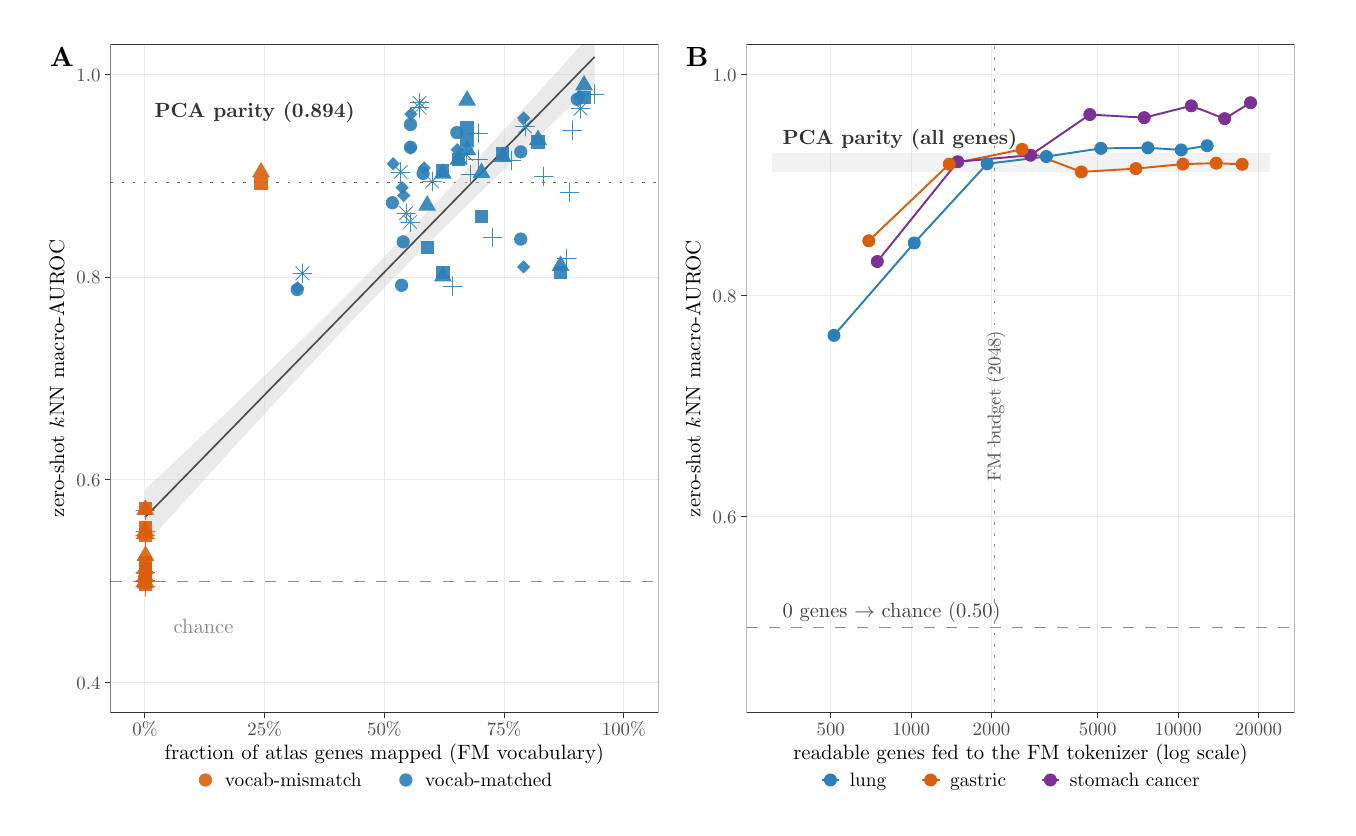
\begin{tikzpicture}[x=1pt,y=1pt]
\definecolor{fillColor}{RGB}{255,255,255}
\path[use as bounding box,fill=fillColor,fill opacity=0.00] (0,0) rectangle (469.75,281.85);
\begin{scope}
\path[clip] (  0.00,  0.00) rectangle (469.75,281.85);
\definecolor{drawColor}{RGB}{255,255,255}
\definecolor{fillColor}{RGB}{255,255,255}

\path[draw=drawColor,line width= 0.4pt,line join=round,line cap=round,fill=fillColor] ( -0.00,  0.00) rectangle (469.76,281.85);
\end{scope}
\begin{scope}
\path[clip] (  4.00,  3.00) rectangle (233.88,278.85);
\definecolor{drawColor}{RGB}{255,255,255}
\definecolor{fillColor}{RGB}{255,255,255}

\path[draw=drawColor,line width= 0.4pt,line join=round,line cap=round,fill=fillColor] (  4.00,  3.00) rectangle (233.88,278.85);
\end{scope}
\begin{scope}
\path[clip] (233.88,  3.00) rectangle (463.76,278.85);
\definecolor{drawColor}{RGB}{255,255,255}
\definecolor{fillColor}{RGB}{255,255,255}

\path[draw=drawColor,line width= 0.4pt,line join=round,line cap=round,fill=fillColor] (233.88,  3.00) rectangle (463.75,278.85);
\end{scope}
\begin{scope}
\path[clip] ( 29.91, 34.23) rectangle (227.88,275.85);
\definecolor{fillColor}{RGB}{255,255,255}

\path[fill=fillColor] ( 29.91, 34.23) rectangle (227.88,275.85);
\definecolor{drawColor}{gray}{0.92}

\path[draw=drawColor,line width= 0.4pt,line join=round] ( 29.91, 45.21) --
	(227.88, 45.21);

\path[draw=drawColor,line width= 0.4pt,line join=round] ( 29.91,118.43) --
	(227.88,118.43);

\path[draw=drawColor,line width= 0.4pt,line join=round] ( 29.91,191.65) --
	(227.88,191.65);

\path[draw=drawColor,line width= 0.4pt,line join=round] ( 29.91,264.87) --
	(227.88,264.87);

\path[draw=drawColor,line width= 0.4pt,line join=round] ( 42.37, 34.23) --
	( 42.37,275.85);

\path[draw=drawColor,line width= 0.4pt,line join=round] ( 85.63, 34.23) --
	( 85.63,275.85);

\path[draw=drawColor,line width= 0.4pt,line join=round] (128.89, 34.23) --
	(128.89,275.85);

\path[draw=drawColor,line width= 0.4pt,line join=round] (172.16, 34.23) --
	(172.16,275.85);

\path[draw=drawColor,line width= 0.4pt,line join=round] (215.42, 34.23) --
	(215.42,275.85);
\definecolor{drawColor}{gray}{0.55}

\path[draw=drawColor,line width= 0.4pt,dash pattern=on 4pt off 4pt ,line join=round] ( 29.91, 81.82) -- (227.88, 81.82);
\definecolor{drawColor}{gray}{0.40}

\path[draw=drawColor,line width= 0.4pt,dash pattern=on 1pt off 3pt ,line join=round] ( 29.91,226.06) -- (227.88,226.06);
\definecolor{fillColor}{RGB}{204,204,204}

\path[fill=fillColor,fill opacity=0.40] ( 42.37,114.85) --
	( 44.43,116.79) --
	( 46.48,118.73) --
	( 48.54,120.67) --
	( 50.60,122.62) --
	( 52.65,124.56) --
	( 54.71,126.51) --
	( 56.77,128.45) --
	( 58.82,130.40) --
	( 60.88,132.36) --
	( 62.94,134.31) --
	( 65.00,136.27) --
	( 67.05,138.22) --
	( 69.11,140.18) --
	( 71.17,142.15) --
	( 73.22,144.11) --
	( 75.28,146.08) --
	( 77.34,148.06) --
	( 79.39,150.03) --
	( 81.45,152.01) --
	( 83.51,153.99) --
	( 85.56,155.98) --
	( 87.62,157.97) --
	( 89.68,159.96) --
	( 91.73,161.96) --
	( 93.79,163.96) --
	( 95.85,165.97) --
	( 97.90,167.98) --
	( 99.96,170.00) --
	(102.02,172.03) --
	(104.08,174.06) --
	(106.13,176.09) --
	(108.19,178.13) --
	(110.25,180.18) --
	(112.30,182.24) --
	(114.36,184.30) --
	(116.42,186.37) --
	(118.47,188.45) --
	(120.53,190.53) --
	(122.59,192.62) --
	(124.64,194.72) --
	(126.70,196.82) --
	(128.76,198.94) --
	(130.81,201.06) --
	(132.87,203.18) --
	(134.93,205.32) --
	(136.99,207.46) --
	(139.04,209.61) --
	(141.10,211.76) --
	(143.16,213.93) --
	(145.21,216.10) --
	(147.27,218.27) --
	(149.33,220.45) --
	(151.38,222.64) --
	(153.44,224.83) --
	(155.50,227.03) --
	(157.55,229.23) --
	(159.61,231.44) --
	(161.67,233.66) --
	(163.72,235.87) --
	(165.78,238.10) --
	(167.84,240.32) --
	(169.90,242.55) --
	(171.95,244.78) --
	(174.01,247.02) --
	(176.07,249.26) --
	(178.12,251.50) --
	(180.18,253.75) --
	(182.24,256.00) --
	(184.29,258.25) --
	(186.35,260.50) --
	(188.41,262.76) --
	(190.46,265.02) --
	(192.52,267.28) --
	(194.58,269.54) --
	(196.63,271.81) --
	(198.69,274.07) --
	(200.75,276.34) --
	(202.81,278.61) --
	(204.86,280.88) --
	(204.86,261.71) --
	(202.81,259.77) --
	(200.75,257.83) --
	(198.69,255.88) --
	(196.63,253.93) --
	(194.58,251.99) --
	(192.52,250.04) --
	(190.46,248.08) --
	(188.41,246.13) --
	(186.35,244.17) --
	(184.29,242.21) --
	(182.24,240.25) --
	(180.18,238.29) --
	(178.12,236.32) --
	(176.07,234.35) --
	(174.01,232.38) --
	(171.95,230.40) --
	(169.90,228.42) --
	(167.84,226.44) --
	(165.78,224.45) --
	(163.72,222.46) --
	(161.67,220.46) --
	(159.61,218.46) --
	(157.55,216.46) --
	(155.50,214.45) --
	(153.44,212.43) --
	(151.38,210.41) --
	(149.33,208.39) --
	(147.27,206.35) --
	(145.21,204.32) --
	(143.16,202.27) --
	(141.10,200.22) --
	(139.04,198.16) --
	(136.99,196.10) --
	(134.93,194.03) --
	(132.87,191.95) --
	(130.81,189.86) --
	(128.76,187.77) --
	(126.70,185.67) --
	(124.64,183.56) --
	(122.59,181.45) --
	(120.53,179.33) --
	(118.47,177.20) --
	(116.42,175.06) --
	(114.36,172.91) --
	(112.30,170.76) --
	(110.25,168.60) --
	(108.19,166.44) --
	(106.13,164.27) --
	(104.08,162.09) --
	(102.02,159.91) --
	( 99.96,157.72) --
	( 97.90,155.52) --
	( 95.85,153.32) --
	( 93.79,151.12) --
	( 91.73,148.91) --
	( 89.68,146.69) --
	( 87.62,144.48) --
	( 85.56,142.25) --
	( 83.51,140.03) --
	( 81.45,137.79) --
	( 79.39,135.56) --
	( 77.34,133.32) --
	( 75.28,131.08) --
	( 73.22,128.84) --
	( 71.17,126.59) --
	( 69.11,124.34) --
	( 67.05,122.09) --
	( 65.00,119.83) --
	( 62.94,117.58) --
	( 60.88,115.32) --
	( 58.82,113.05) --
	( 56.77,110.79) --
	( 54.71,108.53) --
	( 52.65,106.26) --
	( 50.60,103.99) --
	( 48.54,101.72) --
	( 46.48, 99.45) --
	( 44.43, 97.17) --
	( 42.37, 94.90) --
	cycle;

\path[] ( 42.37,114.85) --
	( 44.43,116.79) --
	( 46.48,118.73) --
	( 48.54,120.67) --
	( 50.60,122.62) --
	( 52.65,124.56) --
	( 54.71,126.51) --
	( 56.77,128.45) --
	( 58.82,130.40) --
	( 60.88,132.36) --
	( 62.94,134.31) --
	( 65.00,136.27) --
	( 67.05,138.22) --
	( 69.11,140.18) --
	( 71.17,142.15) --
	( 73.22,144.11) --
	( 75.28,146.08) --
	( 77.34,148.06) --
	( 79.39,150.03) --
	( 81.45,152.01) --
	( 83.51,153.99) --
	( 85.56,155.98) --
	( 87.62,157.97) --
	( 89.68,159.96) --
	( 91.73,161.96) --
	( 93.79,163.96) --
	( 95.85,165.97) --
	( 97.90,167.98) --
	( 99.96,170.00) --
	(102.02,172.03) --
	(104.08,174.06) --
	(106.13,176.09) --
	(108.19,178.13) --
	(110.25,180.18) --
	(112.30,182.24) --
	(114.36,184.30) --
	(116.42,186.37) --
	(118.47,188.45) --
	(120.53,190.53) --
	(122.59,192.62) --
	(124.64,194.72) --
	(126.70,196.82) --
	(128.76,198.94) --
	(130.81,201.06) --
	(132.87,203.18) --
	(134.93,205.32) --
	(136.99,207.46) --
	(139.04,209.61) --
	(141.10,211.76) --
	(143.16,213.93) --
	(145.21,216.10) --
	(147.27,218.27) --
	(149.33,220.45) --
	(151.38,222.64) --
	(153.44,224.83) --
	(155.50,227.03) --
	(157.55,229.23) --
	(159.61,231.44) --
	(161.67,233.66) --
	(163.72,235.87) --
	(165.78,238.10) --
	(167.84,240.32) --
	(169.90,242.55) --
	(171.95,244.78) --
	(174.01,247.02) --
	(176.07,249.26) --
	(178.12,251.50) --
	(180.18,253.75) --
	(182.24,256.00) --
	(184.29,258.25) --
	(186.35,260.50) --
	(188.41,262.76) --
	(190.46,265.02) --
	(192.52,267.28) --
	(194.58,269.54) --
	(196.63,271.81) --
	(198.69,274.07) --
	(200.75,276.34) --
	(202.81,278.61) --
	(204.86,280.88);

\path[] (204.86,261.71) --
	(202.81,259.77) --
	(200.75,257.83) --
	(198.69,255.88) --
	(196.63,253.93) --
	(194.58,251.99) --
	(192.52,250.04) --
	(190.46,248.08) --
	(188.41,246.13) --
	(186.35,244.17) --
	(184.29,242.21) --
	(182.24,240.25) --
	(180.18,238.29) --
	(178.12,236.32) --
	(176.07,234.35) --
	(174.01,232.38) --
	(171.95,230.40) --
	(169.90,228.42) --
	(167.84,226.44) --
	(165.78,224.45) --
	(163.72,222.46) --
	(161.67,220.46) --
	(159.61,218.46) --
	(157.55,216.46) --
	(155.50,214.45) --
	(153.44,212.43) --
	(151.38,210.41) --
	(149.33,208.39) --
	(147.27,206.35) --
	(145.21,204.32) --
	(143.16,202.27) --
	(141.10,200.22) --
	(139.04,198.16) --
	(136.99,196.10) --
	(134.93,194.03) --
	(132.87,191.95) --
	(130.81,189.86) --
	(128.76,187.77) --
	(126.70,185.67) --
	(124.64,183.56) --
	(122.59,181.45) --
	(120.53,179.33) --
	(118.47,177.20) --
	(116.42,175.06) --
	(114.36,172.91) --
	(112.30,170.76) --
	(110.25,168.60) --
	(108.19,166.44) --
	(106.13,164.27) --
	(104.08,162.09) --
	(102.02,159.91) --
	( 99.96,157.72) --
	( 97.90,155.52) --
	( 95.85,153.32) --
	( 93.79,151.12) --
	( 91.73,148.91) --
	( 89.68,146.69) --
	( 87.62,144.48) --
	( 85.56,142.25) --
	( 83.51,140.03) --
	( 81.45,137.79) --
	( 79.39,135.56) --
	( 77.34,133.32) --
	( 75.28,131.08) --
	( 73.22,128.84) --
	( 71.17,126.59) --
	( 69.11,124.34) --
	( 67.05,122.09) --
	( 65.00,119.83) --
	( 62.94,117.58) --
	( 60.88,115.32) --
	( 58.82,113.05) --
	( 56.77,110.79) --
	( 54.71,108.53) --
	( 52.65,106.26) --
	( 50.60,103.99) --
	( 48.54,101.72) --
	( 46.48, 99.45) --
	( 44.43, 97.17) --
	( 42.37, 94.90);
\definecolor{drawColor}{gray}{0.30}

\path[draw=drawColor,line width= 0.6pt,line join=round] ( 42.37,104.88) --
	( 44.43,106.98) --
	( 46.48,109.09) --
	( 48.54,111.20) --
	( 50.60,113.30) --
	( 52.65,115.41) --
	( 54.71,117.52) --
	( 56.77,119.62) --
	( 58.82,121.73) --
	( 60.88,123.84) --
	( 62.94,125.94) --
	( 65.00,128.05) --
	( 67.05,130.16) --
	( 69.11,132.26) --
	( 71.17,134.37) --
	( 73.22,136.48) --
	( 75.28,138.58) --
	( 77.34,140.69) --
	( 79.39,142.80) --
	( 81.45,144.90) --
	( 83.51,147.01) --
	( 85.56,149.11) --
	( 87.62,151.22) --
	( 89.68,153.33) --
	( 91.73,155.43) --
	( 93.79,157.54) --
	( 95.85,159.65) --
	( 97.90,161.75) --
	( 99.96,163.86) --
	(102.02,165.97) --
	(104.08,168.07) --
	(106.13,170.18) --
	(108.19,172.29) --
	(110.25,174.39) --
	(112.30,176.50) --
	(114.36,178.61) --
	(116.42,180.71) --
	(118.47,182.82) --
	(120.53,184.93) --
	(122.59,187.03) --
	(124.64,189.14) --
	(126.70,191.25) --
	(128.76,193.35) --
	(130.81,195.46) --
	(132.87,197.57) --
	(134.93,199.67) --
	(136.99,201.78) --
	(139.04,203.89) --
	(141.10,205.99) --
	(143.16,208.10) --
	(145.21,210.21) --
	(147.27,212.31) --
	(149.33,214.42) --
	(151.38,216.53) --
	(153.44,218.63) --
	(155.50,220.74) --
	(157.55,222.85) --
	(159.61,224.95) --
	(161.67,227.06) --
	(163.72,229.17) --
	(165.78,231.27) --
	(167.84,233.38) --
	(169.90,235.49) --
	(171.95,237.59) --
	(174.01,239.70) --
	(176.07,241.81) --
	(178.12,243.91) --
	(180.18,246.02) --
	(182.24,248.13) --
	(184.29,250.23) --
	(186.35,252.34) --
	(188.41,254.44) --
	(190.46,256.55) --
	(192.52,258.66) --
	(194.58,260.76) --
	(196.63,262.87) --
	(198.69,264.98) --
	(200.75,267.08) --
	(202.81,269.19) --
	(204.86,271.30);
\definecolor{drawColor}{RGB}{44,127,184}

\path[draw=drawColor,draw opacity=0.90,line width= 0.3pt,line join=round,line cap=round] (193.35,244.81) -- (200.14,244.81);

\path[draw=drawColor,draw opacity=0.90,line width= 0.3pt,line join=round,line cap=round] (196.75,241.41) -- (196.75,248.20);
\definecolor{fillColor}{RGB}{44,127,184}

\path[fill=fillColor,fill opacity=0.90] (184.43,245.06) --
	(187.66,239.46) --
	(181.19,239.46) --
	cycle;

\path[fill=fillColor,fill opacity=0.90] (182.02,238.16) --
	(186.83,238.16) --
	(186.83,242.96) --
	(182.02,242.96) --
	cycle;

\path[fill=fillColor,fill opacity=0.90] (176.85,249.24) --
	(179.25,251.64) --
	(181.65,249.24) --
	(179.25,246.84) --
	cycle;

\path[fill=fillColor,fill opacity=0.90] (178.18,236.97) circle (  2.40);

\path[draw=drawColor,draw opacity=0.90,line width= 0.3pt,line join=round,line cap=round] (177.32,243.73) -- (182.12,248.53);

\path[draw=drawColor,draw opacity=0.90,line width= 0.3pt,line join=round,line cap=round] (177.32,248.53) -- (182.12,243.73);

\path[draw=drawColor,draw opacity=0.90,line width= 0.3pt,line join=round,line cap=round] (176.32,246.13) -- (183.11,246.13);

\path[draw=drawColor,draw opacity=0.90,line width= 0.3pt,line join=round,line cap=round] (179.72,242.73) -- (179.72,249.52);

\path[draw=drawColor,draw opacity=0.90,line width= 0.3pt,line join=round,line cap=round] (191.40,198.42) -- (198.19,198.42);

\path[draw=drawColor,draw opacity=0.90,line width= 0.3pt,line join=round,line cap=round] (194.79,195.03) -- (194.79,201.82);

\path[fill=fillColor,fill opacity=0.90] (192.54,199.56) --
	(195.77,193.96) --
	(189.31,193.96) --
	cycle;

\path[fill=fillColor,fill opacity=0.90] (190.14,191.01) --
	(194.94,191.01) --
	(194.94,195.81) --
	(190.14,195.81) --
	cycle;

\path[fill=fillColor,fill opacity=0.90] (176.80,195.42) --
	(179.20,197.82) --
	(181.60,195.42) --
	(179.20,193.02) --
	cycle;

\path[fill=fillColor,fill opacity=0.90] (178.16,205.45) circle (  2.40);
\definecolor{drawColor}{RGB}{217,95,14}

\path[draw=drawColor,draw opacity=0.90,line width= 0.3pt,line join=round,line cap=round] ( 39.18, 99.98) -- ( 45.97, 99.98);

\path[draw=drawColor,draw opacity=0.90,line width= 0.3pt,line join=round,line cap=round] ( 42.58, 96.58) -- ( 42.58,103.37);
\definecolor{fillColor}{RGB}{217,95,14}

\path[fill=fillColor,fill opacity=0.90] ( 42.58, 94.78) --
	( 45.81, 89.18) --
	( 39.34, 89.18) --
	cycle;

\path[fill=fillColor,fill opacity=0.90] ( 40.18, 86.08) --
	( 44.98, 86.08) --
	( 44.98, 90.88) --
	( 40.18, 90.88) --
	cycle;
\definecolor{drawColor}{RGB}{44,127,184}

\path[draw=drawColor,draw opacity=0.90,line width= 0.3pt,line join=round,line cap=round] (150.24,188.39) -- (157.03,188.39);

\path[draw=drawColor,draw opacity=0.90,line width= 0.3pt,line join=round,line cap=round] (153.64,185.00) -- (153.64,191.79);
\definecolor{fillColor}{RGB}{44,127,184}

\path[fill=fillColor,fill opacity=0.90] (150.06,195.75) --
	(153.29,190.15) --
	(146.82,190.15) --
	cycle;

\path[fill=fillColor,fill opacity=0.90] (147.66,191.01) --
	(152.46,191.01) --
	(152.46,195.81) --
	(147.66,195.81) --
	cycle;

\path[fill=fillColor,fill opacity=0.90] ( 95.14,187.84) --
	( 97.54,190.24) --
	( 99.94,187.84) --
	( 97.54,185.44) --
	cycle;

\path[fill=fillColor,fill opacity=0.90] ( 97.40,187.22) circle (  2.40);

\path[draw=drawColor,draw opacity=0.90,line width= 0.3pt,line join=round,line cap=round] ( 96.87,190.68) -- (101.67,195.48);

\path[draw=drawColor,draw opacity=0.90,line width= 0.3pt,line join=round,line cap=round] ( 96.87,195.48) -- (101.67,190.68);

\path[draw=drawColor,draw opacity=0.90,line width= 0.3pt,line join=round,line cap=round] ( 95.87,193.08) -- (102.66,193.08);

\path[draw=drawColor,draw opacity=0.90,line width= 0.3pt,line join=round,line cap=round] ( 99.27,189.68) -- ( 99.27,196.47);

\path[draw=drawColor,draw opacity=0.90,line width= 0.3pt,line join=round,line cap=round] (192.42,222.33) -- (199.21,222.33);

\path[draw=drawColor,draw opacity=0.90,line width= 0.3pt,line join=round,line cap=round] (195.81,218.93) -- (195.81,225.72);

\path[fill=fillColor,fill opacity=0.90] (150.02,232.87) --
	(153.26,227.27) --
	(146.79,227.27) --
	cycle;

\path[fill=fillColor,fill opacity=0.90] (147.62,227.80) --
	(152.42,227.80) --
	(152.42,232.60) --
	(147.62,232.60) --
	cycle;

\path[fill=fillColor,fill opacity=0.90] (132.90,224.05) --
	(135.30,226.45) --
	(137.70,224.05) --
	(135.30,221.65) --
	cycle;

\path[fill=fillColor,fill opacity=0.90] (135.11,188.76) circle (  2.40);

\path[draw=drawColor,draw opacity=0.90,line width= 0.3pt,line join=round,line cap=round] (135.82,209.24) -- (140.62,214.04);

\path[draw=drawColor,draw opacity=0.90,line width= 0.3pt,line join=round,line cap=round] (135.82,214.04) -- (140.62,209.24);

\path[draw=drawColor,draw opacity=0.90,line width= 0.3pt,line join=round,line cap=round] (134.83,211.64) -- (141.62,211.64);

\path[draw=drawColor,draw opacity=0.90,line width= 0.3pt,line join=round,line cap=round] (138.22,208.24) -- (138.22,215.03);
\definecolor{drawColor}{RGB}{217,95,14}

\path[draw=drawColor,draw opacity=0.90,line width= 0.3pt,line join=round,line cap=round] ( 39.10,107.48) -- ( 45.89,107.48);

\path[draw=drawColor,draw opacity=0.90,line width= 0.3pt,line join=round,line cap=round] ( 42.49,104.09) -- ( 42.49,110.88);
\definecolor{fillColor}{RGB}{217,95,14}

\path[fill=fillColor,fill opacity=0.90] ( 42.49,111.40) --
	( 45.72,105.80) --
	( 39.26,105.80) --
	cycle;

\path[fill=fillColor,fill opacity=0.90] ( 40.09,105.63) --
	( 44.89,105.63) --
	( 44.89,110.43) --
	( 40.09,110.43) --
	cycle;
\definecolor{drawColor}{RGB}{44,127,184}

\path[draw=drawColor,draw opacity=0.90,line width= 0.3pt,line join=round,line cap=round] (183.12,228.11) -- (189.91,228.11);

\path[draw=drawColor,draw opacity=0.90,line width= 0.3pt,line join=round,line cap=round] (186.52,224.72) -- (186.52,231.51);
\definecolor{fillColor}{RGB}{44,127,184}

\path[fill=fillColor,fill opacity=0.90] (144.35,221.34) --
	(147.58,215.74) --
	(141.11,215.74) --
	cycle;

\path[fill=fillColor,fill opacity=0.90] (141.95,200.01) --
	(146.75,200.01) --
	(146.75,204.81) --
	(141.95,204.81) --
	cycle;

\path[fill=fillColor,fill opacity=0.90] (133.50,221.19) --
	(135.90,223.60) --
	(138.30,221.19) --
	(135.90,218.79) --
	cycle;

\path[fill=fillColor,fill opacity=0.90] (135.69,204.46) circle (  2.40);

\path[draw=drawColor,draw opacity=0.90,line width= 0.3pt,line join=round,line cap=round] (134.35,212.42) -- (139.15,217.23);

\path[draw=drawColor,draw opacity=0.90,line width= 0.3pt,line join=round,line cap=round] (134.35,217.23) -- (139.15,212.42);

\path[draw=drawColor,draw opacity=0.90,line width= 0.3pt,line join=round,line cap=round] (133.36,214.82) -- (140.15,214.82);

\path[draw=drawColor,draw opacity=0.90,line width= 0.3pt,line join=round,line cap=round] (136.75,211.43) -- (136.75,218.22);
\definecolor{drawColor}{RGB}{217,95,14}

\path[draw=drawColor,draw opacity=0.90,line width= 0.3pt,line join=round,line cap=round] ( 39.06, 98.22) -- ( 45.85, 98.22);

\path[draw=drawColor,draw opacity=0.90,line width= 0.3pt,line join=round,line cap=round] ( 42.46, 94.83) -- ( 42.46,101.62);
\definecolor{fillColor}{RGB}{217,95,14}

\path[fill=fillColor,fill opacity=0.90] ( 42.46,102.80) --
	( 45.69, 97.20) --
	( 39.22, 97.20) --
	cycle;

\path[fill=fillColor,fill opacity=0.90] ( 40.06, 98.60) --
	( 44.86, 98.60) --
	( 44.86,103.41) --
	( 40.06,103.41) --
	cycle;
\definecolor{drawColor}{RGB}{44,127,184}

\path[draw=drawColor,draw opacity=0.90,line width= 0.3pt,line join=round,line cap=round] (156.60,228.70) -- (163.39,228.70);

\path[draw=drawColor,draw opacity=0.90,line width= 0.3pt,line join=round,line cap=round] (159.99,225.30) -- (159.99,232.09);
\definecolor{fillColor}{RGB}{44,127,184}

\path[fill=fillColor,fill opacity=0.90] (155.66,237.92) --
	(158.90,232.32) --
	(152.43,232.32) --
	cycle;

\path[fill=fillColor,fill opacity=0.90] (153.26,231.79) --
	(158.06,231.79) --
	(158.06,236.59) --
	(153.26,236.59) --
	cycle;

\path[fill=fillColor,fill opacity=0.90] (129.68,232.69) --
	(132.08,235.09) --
	(134.48,232.69) --
	(132.08,230.29) --
	cycle;

\path[fill=fillColor,fill opacity=0.90] (131.78,218.60) circle (  2.40);

\path[draw=drawColor,draw opacity=0.90,line width= 0.3pt,line join=round,line cap=round] (132.38,227.29) -- (137.18,232.09);

\path[draw=drawColor,draw opacity=0.90,line width= 0.3pt,line join=round,line cap=round] (132.38,232.09) -- (137.18,227.29);

\path[draw=drawColor,draw opacity=0.90,line width= 0.3pt,line join=round,line cap=round] (131.38,229.69) -- (138.17,229.69);

\path[draw=drawColor,draw opacity=0.90,line width= 0.3pt,line join=round,line cap=round] (134.78,226.29) -- (134.78,233.08);

\path[draw=drawColor,draw opacity=0.90,line width= 0.3pt,line join=round,line cap=round] (164.66,206.00) -- (171.45,206.00);

\path[draw=drawColor,draw opacity=0.90,line width= 0.3pt,line join=round,line cap=round] (168.05,202.61) -- (168.05,209.40);

\path[fill=fillColor,fill opacity=0.90] (163.99,233.13) --
	(167.22,227.53) --
	(160.75,227.53) --
	cycle;

\path[fill=fillColor,fill opacity=0.90] (161.59,211.22) --
	(166.39,211.22) --
	(166.39,216.02) --
	(161.59,216.02) --
	cycle;

\path[fill=fillColor,fill opacity=0.90] (140.91,231.15) --
	(143.31,233.55) --
	(145.71,231.15) --
	(143.31,228.75) --
	cycle;

\path[fill=fillColor,fill opacity=0.90] (142.89,229.18) circle (  2.40);

\path[draw=drawColor,draw opacity=0.90,line width= 0.3pt,line join=round,line cap=round] (143.73,223.88) -- (148.53,228.68);

\path[draw=drawColor,draw opacity=0.90,line width= 0.3pt,line join=round,line cap=round] (143.73,228.68) -- (148.53,223.88);

\path[draw=drawColor,draw opacity=0.90,line width= 0.3pt,line join=round,line cap=round] (142.73,226.28) -- (149.52,226.28);

\path[draw=drawColor,draw opacity=0.90,line width= 0.3pt,line join=round,line cap=round] (146.13,222.89) -- (146.13,229.68);

\path[draw=drawColor,draw opacity=0.90,line width= 0.3pt,line join=round,line cap=round] (159.33,243.75) -- (166.12,243.75);

\path[draw=drawColor,draw opacity=0.90,line width= 0.3pt,line join=round,line cap=round] (162.72,240.35) -- (162.72,247.14);

\path[fill=fillColor,fill opacity=0.90] (158.78,241.48) --
	(162.01,235.88) --
	(155.55,235.88) --
	cycle;

\path[fill=fillColor,fill opacity=0.90] (156.38,238.67) --
	(161.18,238.67) --
	(161.18,243.47) --
	(156.38,243.47) --
	cycle;

\path[fill=fillColor,fill opacity=0.90] (136.08,238.33) --
	(138.48,240.73) --
	(140.88,238.33) --
	(138.48,235.93) --
	cycle;

\path[fill=fillColor,fill opacity=0.90] (138.34,238.62) circle (  2.40);

\path[draw=drawColor,draw opacity=0.90,line width= 0.3pt,line join=round,line cap=round] (139.23,250.50) -- (144.03,255.30);

\path[draw=drawColor,draw opacity=0.90,line width= 0.3pt,line join=round,line cap=round] (139.23,255.30) -- (144.03,250.50);

\path[draw=drawColor,draw opacity=0.90,line width= 0.3pt,line join=round,line cap=round] (138.24,252.90) -- (145.03,252.90);

\path[draw=drawColor,draw opacity=0.90,line width= 0.3pt,line join=round,line cap=round] (141.63,249.50) -- (141.63,256.29);

\path[draw=drawColor,draw opacity=0.90,line width= 0.3pt,line join=round,line cap=round] (171.36,233.82) -- (178.15,233.82);

\path[draw=drawColor,draw opacity=0.90,line width= 0.3pt,line join=round,line cap=round] (174.75,230.43) -- (174.75,237.22);

\path[fill=fillColor,fill opacity=0.90] (171.65,238.91) --
	(174.89,233.31) --
	(168.42,233.31) --
	cycle;

\path[fill=fillColor,fill opacity=0.90] (169.25,234.06) --
	(174.05,234.06) --
	(174.05,238.86) --
	(169.25,238.86) --
	cycle;

\path[fill=fillColor,fill opacity=0.90] (152.83,237.71) --
	(155.23,240.11) --
	(157.63,237.71) --
	(155.23,235.30) --
	cycle;

\path[fill=fillColor,fill opacity=0.90] (155.08,243.93) circle (  2.40);

\path[draw=drawColor,draw opacity=0.90,line width= 0.3pt,line join=round,line cap=round] (156.08,233.69) -- (160.89,238.50);

\path[draw=drawColor,draw opacity=0.90,line width= 0.3pt,line join=round,line cap=round] (156.08,238.50) -- (160.89,233.69);

\path[draw=drawColor,draw opacity=0.90,line width= 0.3pt,line join=round,line cap=round] (155.09,236.09) -- (161.88,236.09);

\path[draw=drawColor,draw opacity=0.90,line width= 0.3pt,line join=round,line cap=round] (158.49,232.70) -- (158.49,239.49);
\definecolor{drawColor}{RGB}{217,95,14}

\path[draw=drawColor,draw opacity=0.90,line width= 0.3pt,line join=round,line cap=round] ( 38.97, 81.82) -- ( 45.76, 81.82);

\path[draw=drawColor,draw opacity=0.90,line width= 0.3pt,line join=round,line cap=round] ( 42.37, 78.43) -- ( 42.37, 85.22);
\definecolor{fillColor}{RGB}{217,95,14}

\path[fill=fillColor,fill opacity=0.90] ( 84.32,233.35) --
	( 87.55,227.75) --
	( 81.08,227.75) --
	cycle;

\path[fill=fillColor,fill opacity=0.90] ( 81.92,223.26) --
	( 86.72,223.26) --
	( 86.72,228.06) --
	( 81.92,228.06) --
	cycle;

\path[draw=drawColor,draw opacity=0.90,line width= 0.3pt,line join=round,line cap=round] ( 38.97, 81.82) -- ( 45.76, 81.82);

\path[draw=drawColor,draw opacity=0.90,line width= 0.3pt,line join=round,line cap=round] ( 42.37, 78.43) -- ( 42.37, 85.22);

\path[fill=fillColor,fill opacity=0.90] ( 42.37, 85.55) --
	( 45.60, 79.95) --
	( 39.14, 79.95) --
	cycle;

\path[fill=fillColor,fill opacity=0.90] ( 39.97, 79.42) --
	( 44.77, 79.42) --
	( 44.77, 84.22) --
	( 39.97, 84.22) --
	cycle;

\path[draw=drawColor,draw opacity=0.90,line width= 0.3pt,line join=round,line cap=round] ( 39.08, 79.77) -- ( 45.87, 79.77);

\path[draw=drawColor,draw opacity=0.90,line width= 0.3pt,line join=round,line cap=round] ( 42.47, 76.38) -- ( 42.47, 83.17);

\path[fill=fillColor,fill opacity=0.90] ( 42.47, 84.82) --
	( 45.71, 79.22) --
	( 39.24, 79.22) --
	cycle;

\path[fill=fillColor,fill opacity=0.90] ( 40.07, 78.40) --
	( 44.87, 78.40) --
	( 44.87, 83.20) --
	( 40.07, 83.20) --
	cycle;
\definecolor{drawColor}{RGB}{44,127,184}

\path[draw=drawColor,draw opacity=0.90,line width= 0.3pt,line join=round,line cap=round] (201.47,257.88) -- (208.26,257.88);

\path[draw=drawColor,draw opacity=0.90,line width= 0.3pt,line join=round,line cap=round] (204.86,254.48) -- (204.86,261.27);
\definecolor{fillColor}{RGB}{44,127,184}

\path[fill=fillColor,fill opacity=0.90] (201.04,264.80) --
	(204.27,259.20) --
	(197.80,259.20) --
	cycle;

\path[fill=fillColor,fill opacity=0.90] (198.64,254.27) --
	(203.44,254.27) --
	(203.44,259.07) --
	(198.64,259.07) --
	cycle;

\path[fill=fillColor,fill opacity=0.90] (197.01,257.07) --
	(199.41,259.47) --
	(201.81,257.07) --
	(199.41,254.67) --
	cycle;

\path[fill=fillColor,fill opacity=0.90] (198.60,255.97) circle (  2.40);

\path[draw=drawColor,draw opacity=0.90,line width= 0.3pt,line join=round,line cap=round] (197.41,250.17) -- (202.21,254.97);

\path[draw=drawColor,draw opacity=0.90,line width= 0.3pt,line join=round,line cap=round] (197.41,254.97) -- (202.21,250.17);

\path[draw=drawColor,draw opacity=0.90,line width= 0.3pt,line join=round,line cap=round] (196.41,252.57) -- (203.20,252.57);

\path[draw=drawColor,draw opacity=0.90,line width= 0.3pt,line join=round,line cap=round] (199.81,249.17) -- (199.81,255.96);
\definecolor{drawColor}{RGB}{217,95,14}

\path[draw=drawColor,draw opacity=0.90,line width= 0.3pt,line join=round,line cap=round] ( 39.06, 82.26) -- ( 45.85, 82.26);

\path[draw=drawColor,draw opacity=0.90,line width= 0.3pt,line join=round,line cap=round] ( 42.46, 78.87) -- ( 42.46, 85.66);
\definecolor{fillColor}{RGB}{217,95,14}

\path[fill=fillColor,fill opacity=0.90] ( 42.46, 90.09) --
	( 45.69, 84.49) --
	( 39.22, 84.49) --
	cycle;

\path[fill=fillColor,fill opacity=0.90] ( 40.06, 83.96) --
	( 44.86, 83.96) --
	( 44.86, 88.76) --
	( 40.06, 88.76) --
	cycle;
\definecolor{drawColor}{RGB}{44,127,184}

\path[draw=drawColor,draw opacity=0.90,line width= 0.3pt,line join=round,line cap=round] (159.33,234.34) -- (166.12,234.34);

\path[draw=drawColor,draw opacity=0.90,line width= 0.3pt,line join=round,line cap=round] (162.72,230.94) -- (162.72,237.73);
\definecolor{fillColor}{RGB}{44,127,184}

\path[fill=fillColor,fill opacity=0.90] (158.78,259.30) --
	(162.01,253.70) --
	(155.55,253.70) --
	cycle;

\path[fill=fillColor,fill opacity=0.90] (156.38,243.36) --
	(161.18,243.36) --
	(161.18,248.16) --
	(156.38,248.16) --
	cycle;

\path[fill=fillColor,fill opacity=0.90] (136.08,250.63) --
	(138.48,253.03) --
	(140.88,250.63) --
	(138.48,248.23) --
	cycle;

\path[fill=fillColor,fill opacity=0.90] (138.34,246.86) circle (  2.40);

\path[draw=drawColor,draw opacity=0.90,line width= 0.3pt,line join=round,line cap=round] (139.23,252.29) -- (144.03,257.09);

\path[draw=drawColor,draw opacity=0.90,line width= 0.3pt,line join=round,line cap=round] (139.23,257.09) -- (144.03,252.29);

\path[draw=drawColor,draw opacity=0.90,line width= 0.3pt,line join=round,line cap=round] (138.24,254.69) -- (145.03,254.69);

\path[draw=drawColor,draw opacity=0.90,line width= 0.3pt,line join=round,line cap=round] (141.63,251.30) -- (141.63,258.09);
\definecolor{drawColor}{RGB}{217,95,14}

\path[draw=drawColor,draw opacity=0.90,line width= 0.3pt,line join=round,line cap=round] ( 39.08, 97.45) -- ( 45.87, 97.45);

\path[draw=drawColor,draw opacity=0.90,line width= 0.3pt,line join=round,line cap=round] ( 42.47, 94.06) -- ( 42.47,100.85);
\definecolor{fillColor}{RGB}{217,95,14}

\path[fill=fillColor,fill opacity=0.90] ( 42.47,103.64) --
	( 45.71, 98.04) --
	( 39.24, 98.04) --
	cycle;

\path[fill=fillColor,fill opacity=0.90] ( 40.07, 95.93) --
	( 44.87, 95.93) --
	( 44.87,100.73) --
	( 40.07,100.73) --
	cycle;

\path[draw=drawColor,draw opacity=0.90,line width= 0.3pt,line join=round,line cap=round] ( 39.06, 84.93) -- ( 45.85, 84.93);

\path[draw=drawColor,draw opacity=0.90,line width= 0.3pt,line join=round,line cap=round] ( 42.46, 81.54) -- ( 42.46, 88.33);

\path[fill=fillColor,fill opacity=0.90] ( 42.46, 87.17) --
	( 45.69, 81.57) --
	( 39.22, 81.57) --
	cycle;

\path[fill=fillColor,fill opacity=0.90] ( 40.06, 81.07) --
	( 44.86, 81.07) --
	( 44.86, 85.87) --
	( 40.06, 85.87) --
	cycle;
\definecolor{drawColor}{gray}{0.55}

\node[text=drawColor,anchor=base west,inner sep=0pt, outer sep=0pt, scale=  0.74] at ( 52.75, 62.80) {chance};
\definecolor{drawColor}{gray}{0.20}

\node[text=drawColor,anchor=base west,inner sep=0pt, outer sep=0pt, scale=  0.74] at ( 45.83,249.50) {\bfseries PCA parity (0.894)};

\path[draw=drawColor,line width= 0.4pt,line join=round,line cap=round] ( 29.91, 34.23) rectangle (227.88,275.85);
\end{scope}
\begin{scope}
\path[clip] (  0.00,  0.00) rectangle (469.75,281.85);
\definecolor{drawColor}{gray}{0.30}

\node[text=drawColor,anchor=base east,inner sep=0pt, outer sep=0pt, scale=  0.68] at ( 26.31, 42.87) {0.4};

\node[text=drawColor,anchor=base east,inner sep=0pt, outer sep=0pt, scale=  0.68] at ( 26.31,116.09) {0.6};

\node[text=drawColor,anchor=base east,inner sep=0pt, outer sep=0pt, scale=  0.68] at ( 26.31,189.31) {0.8};

\node[text=drawColor,anchor=base east,inner sep=0pt, outer sep=0pt, scale=  0.68] at ( 26.31,262.53) {1.0};
\end{scope}
\begin{scope}
\path[clip] (  0.00,  0.00) rectangle (469.75,281.85);
\definecolor{drawColor}{gray}{0.20}

\path[draw=drawColor,line width= 0.4pt,line join=round] ( 27.91, 45.21) --
	( 29.91, 45.21);

\path[draw=drawColor,line width= 0.4pt,line join=round] ( 27.91,118.43) --
	( 29.91,118.43);

\path[draw=drawColor,line width= 0.4pt,line join=round] ( 27.91,191.65) --
	( 29.91,191.65);

\path[draw=drawColor,line width= 0.4pt,line join=round] ( 27.91,264.87) --
	( 29.91,264.87);
\end{scope}
\begin{scope}
\path[clip] (  0.00,  0.00) rectangle (469.75,281.85);
\definecolor{drawColor}{gray}{0.20}

\path[draw=drawColor,line width= 0.4pt,line join=round] ( 42.37, 32.23) --
	( 42.37, 34.23);

\path[draw=drawColor,line width= 0.4pt,line join=round] ( 85.63, 32.23) --
	( 85.63, 34.23);

\path[draw=drawColor,line width= 0.4pt,line join=round] (128.89, 32.23) --
	(128.89, 34.23);

\path[draw=drawColor,line width= 0.4pt,line join=round] (172.16, 32.23) --
	(172.16, 34.23);

\path[draw=drawColor,line width= 0.4pt,line join=round] (215.42, 32.23) --
	(215.42, 34.23);
\end{scope}
\begin{scope}
\path[clip] (  0.00,  0.00) rectangle (469.75,281.85);
\definecolor{drawColor}{gray}{0.30}

\node[text=drawColor,anchor=base,inner sep=0pt, outer sep=0pt, scale=  0.68] at ( 42.37, 25.95) {0\%};

\node[text=drawColor,anchor=base,inner sep=0pt, outer sep=0pt, scale=  0.68] at ( 85.63, 25.95) {25\%};

\node[text=drawColor,anchor=base,inner sep=0pt, outer sep=0pt, scale=  0.68] at (128.89, 25.95) {50\%};

\node[text=drawColor,anchor=base,inner sep=0pt, outer sep=0pt, scale=  0.68] at (172.16, 25.95) {75\%};

\node[text=drawColor,anchor=base,inner sep=0pt, outer sep=0pt, scale=  0.68] at (215.42, 25.95) {100\%};
\end{scope}
\begin{scope}
\path[clip] (  0.00,  0.00) rectangle (469.75,281.85);
\definecolor{drawColor}{RGB}{0,0,0}

\node[text=drawColor,anchor=base,inner sep=0pt, outer sep=0pt, scale=  0.75] at (128.89, 17.46) {fraction of atlas genes mapped (FM vocabulary)};
\end{scope}
\begin{scope}
\path[clip] (  0.00,  0.00) rectangle (469.75,281.85);
\definecolor{drawColor}{RGB}{0,0,0}

\node[text=drawColor,rotate= 90.00,anchor=base,inner sep=0pt, outer sep=0pt, scale=  0.75] at ( 13.17,155.04) {zero-shot $k$NN macro-AUROC};
\end{scope}
\begin{scope}
\path[clip] (  0.00,  0.00) rectangle (469.75,281.85);
\definecolor{fillColor}{RGB}{255,255,255}

\path[fill=fillColor] ( 59.25,  6.00) rectangle (198.54, 14.00);
\end{scope}
\begin{scope}
\path[clip] (  0.00,  0.00) rectangle (469.75,281.85);
\definecolor{fillColor}{RGB}{255,255,255}

\path[fill=fillColor] ( 60.25,  6.00) rectangle ( 68.25, 14.00);
\definecolor{fillColor}{RGB}{217,95,14}

\path[fill=fillColor,fill opacity=0.90] ( 64.25, 10.00) circle (  2.40);
\end{scope}
\begin{scope}
\path[clip] (  0.00,  0.00) rectangle (469.75,281.85);
\definecolor{fillColor}{RGB}{255,255,255}

\path[fill=fillColor] (132.66,  6.00) rectangle (140.66, 14.00);
\definecolor{fillColor}{RGB}{44,127,184}

\path[fill=fillColor,fill opacity=0.90] (136.66, 10.00) circle (  2.40);
\end{scope}
\begin{scope}
\path[clip] (  0.00,  0.00) rectangle (469.75,281.85);
\definecolor{drawColor}{RGB}{0,0,0}

\node[text=drawColor,anchor=base west,inner sep=0pt, outer sep=0pt, scale=  0.70] at ( 71.25,  7.59) {vocab-mismatch};
\end{scope}
\begin{scope}
\path[clip] (  0.00,  0.00) rectangle (469.75,281.85);
\definecolor{drawColor}{RGB}{0,0,0}

\node[text=drawColor,anchor=base west,inner sep=0pt, outer sep=0pt, scale=  0.70] at (143.66,  7.59) {vocab-matched};
\end{scope}
\begin{scope}
\path[clip] (  0.00,  0.00) rectangle (469.75,281.85);
\definecolor{drawColor}{RGB}{0,0,0}

\node[text=drawColor,anchor=base,inner sep=0pt, outer sep=0pt, scale=  1.00] at ( 12.35,267.98) {\bfseries A};
\end{scope}
\begin{scope}
\path[clip] (259.79, 34.23) rectangle (457.76,275.85);
\definecolor{fillColor}{RGB}{255,255,255}

\path[fill=fillColor] (259.79, 34.23) rectangle (457.75,275.85);
\definecolor{drawColor}{gray}{0.92}

\path[draw=drawColor,line width= 0.4pt,line join=round] (259.79,105.12) --
	(457.76,105.12);

\path[draw=drawColor,line width= 0.4pt,line join=round] (259.79,184.99) --
	(457.76,184.99);

\path[draw=drawColor,line width= 0.4pt,line join=round] (259.79,264.87) --
	(457.76,264.87);

\path[draw=drawColor,line width= 0.4pt,line join=round] (290.19, 34.23) --
	(290.19,275.85);

\path[draw=drawColor,line width= 0.4pt,line join=round] (319.24, 34.23) --
	(319.24,275.85);

\path[draw=drawColor,line width= 0.4pt,line join=round] (348.28, 34.23) --
	(348.28,275.85);

\path[draw=drawColor,line width= 0.4pt,line join=round] (386.67, 34.23) --
	(386.67,275.85);

\path[draw=drawColor,line width= 0.4pt,line join=round] (415.72, 34.23) --
	(415.72,275.85);

\path[draw=drawColor,line width= 0.4pt,line join=round] (444.76, 34.23) --
	(444.76,275.85);
\definecolor{fillColor}{RGB}{179,179,179}

\path[fill=fillColor,fill opacity=0.16] (268.79,229.68) rectangle (448.76,236.67);
\definecolor{drawColor}{gray}{0.55}

\path[draw=drawColor,line width= 0.4pt,dash pattern=on 4pt off 4pt ,line join=round] (259.79, 65.18) -- (457.76, 65.18);

\path[draw=drawColor,line width= 0.4pt,dash pattern=on 1pt off 3pt ,line join=round] (349.27, 34.23) -- (349.27,275.85);
\definecolor{drawColor}{RGB}{44,127,184}

\path[draw=drawColor,line width= 0.7pt,line join=round] (291.35,170.66) --
	(320.35,204.04) --
	(346.70,232.68) --
	(368.10,235.28) --
	(387.80,238.23) --
	(404.78,238.43) --
	(416.84,237.67) --
	(426.19,239.19);
\definecolor{drawColor}{RGB}{217,95,14}

\path[draw=drawColor,line width= 0.7pt,line join=round] (303.93,204.84) --
	(333.00,232.52) --
	(359.34,237.87) --
	(380.74,229.72) --
	(400.44,230.92) --
	(417.43,232.56) --
	(429.49,232.88) --
	(438.84,232.48);
\definecolor{drawColor}{RGB}{123,50,148}

\path[draw=drawColor,line width= 0.7pt,line join=round] (307.01,197.34) --
	(336.06,233.40) --
	(362.38,235.76) --
	(383.80,250.45) --
	(403.48,249.33) --
	(420.47,253.61) --
	(432.53,248.97) --
	(441.88,254.73);
\definecolor{drawColor}{RGB}{44,127,184}
\definecolor{fillColor}{RGB}{44,127,184}

\path[draw=drawColor,line width= 0.3pt,line join=round,line cap=round,fill=fillColor] (426.19,239.19) circle (  2.19);

\path[draw=drawColor,line width= 0.3pt,line join=round,line cap=round,fill=fillColor] (416.84,237.67) circle (  2.19);

\path[draw=drawColor,line width= 0.3pt,line join=round,line cap=round,fill=fillColor] (404.78,238.43) circle (  2.19);

\path[draw=drawColor,line width= 0.3pt,line join=round,line cap=round,fill=fillColor] (387.80,238.23) circle (  2.19);

\path[draw=drawColor,line width= 0.3pt,line join=round,line cap=round,fill=fillColor] (368.10,235.28) circle (  2.19);

\path[draw=drawColor,line width= 0.3pt,line join=round,line cap=round,fill=fillColor] (346.70,232.68) circle (  2.19);

\path[draw=drawColor,line width= 0.3pt,line join=round,line cap=round,fill=fillColor] (320.35,204.04) circle (  2.19);

\path[draw=drawColor,line width= 0.3pt,line join=round,line cap=round,fill=fillColor] (291.35,170.66) circle (  2.19);
\definecolor{drawColor}{RGB}{123,50,148}
\definecolor{fillColor}{RGB}{123,50,148}

\path[draw=drawColor,line width= 0.3pt,line join=round,line cap=round,fill=fillColor] (441.88,254.73) circle (  2.19);

\path[draw=drawColor,line width= 0.3pt,line join=round,line cap=round,fill=fillColor] (432.53,248.97) circle (  2.19);

\path[draw=drawColor,line width= 0.3pt,line join=round,line cap=round,fill=fillColor] (420.47,253.61) circle (  2.19);

\path[draw=drawColor,line width= 0.3pt,line join=round,line cap=round,fill=fillColor] (403.48,249.33) circle (  2.19);

\path[draw=drawColor,line width= 0.3pt,line join=round,line cap=round,fill=fillColor] (383.80,250.45) circle (  2.19);

\path[draw=drawColor,line width= 0.3pt,line join=round,line cap=round,fill=fillColor] (362.38,235.76) circle (  2.19);

\path[draw=drawColor,line width= 0.3pt,line join=round,line cap=round,fill=fillColor] (336.06,233.40) circle (  2.19);

\path[draw=drawColor,line width= 0.3pt,line join=round,line cap=round,fill=fillColor] (307.01,197.34) circle (  2.19);
\definecolor{drawColor}{RGB}{217,95,14}
\definecolor{fillColor}{RGB}{217,95,14}

\path[draw=drawColor,line width= 0.3pt,line join=round,line cap=round,fill=fillColor] (438.84,232.48) circle (  2.19);

\path[draw=drawColor,line width= 0.3pt,line join=round,line cap=round,fill=fillColor] (429.49,232.88) circle (  2.19);

\path[draw=drawColor,line width= 0.3pt,line join=round,line cap=round,fill=fillColor] (417.43,232.56) circle (  2.19);

\path[draw=drawColor,line width= 0.3pt,line join=round,line cap=round,fill=fillColor] (400.44,230.92) circle (  2.19);

\path[draw=drawColor,line width= 0.3pt,line join=round,line cap=round,fill=fillColor] (380.74,229.72) circle (  2.19);

\path[draw=drawColor,line width= 0.3pt,line join=round,line cap=round,fill=fillColor] (359.34,237.87) circle (  2.19);

\path[draw=drawColor,line width= 0.3pt,line join=round,line cap=round,fill=fillColor] (333.00,232.52) circle (  2.19);

\path[draw=drawColor,line width= 0.3pt,line join=round,line cap=round,fill=fillColor] (303.93,204.84) circle (  2.19);
\definecolor{drawColor}{gray}{0.25}

\node[text=drawColor,anchor=base west,inner sep=0pt, outer sep=0pt, scale=  0.74] at (272.78, 68.62) {0 genes $\to$ chance (0.50)};
\definecolor{drawColor}{gray}{0.35}

\node[text=drawColor,rotate= 90.00,anchor=base,inner sep=0pt, outer sep=0pt, scale=  0.68] at (351.62,145.06) {FM budget (2048)};
\definecolor{drawColor}{gray}{0.20}

\node[text=drawColor,anchor=base west,inner sep=0pt, outer sep=0pt, scale=  0.74] at (272.78,239.71) {\bfseries PCA parity (all genes)};

\path[draw=drawColor,line width= 0.4pt,line join=round,line cap=round] (259.79, 34.23) rectangle (457.75,275.85);
\end{scope}
\begin{scope}
\path[clip] (  0.00,  0.00) rectangle (469.75,281.85);
\definecolor{drawColor}{gray}{0.30}

\node[text=drawColor,anchor=base east,inner sep=0pt, outer sep=0pt, scale=  0.68] at (256.19,102.78) {0.6};

\node[text=drawColor,anchor=base east,inner sep=0pt, outer sep=0pt, scale=  0.68] at (256.19,182.65) {0.8};

\node[text=drawColor,anchor=base east,inner sep=0pt, outer sep=0pt, scale=  0.68] at (256.19,262.53) {1.0};
\end{scope}
\begin{scope}
\path[clip] (  0.00,  0.00) rectangle (469.75,281.85);
\definecolor{drawColor}{gray}{0.20}

\path[draw=drawColor,line width= 0.4pt,line join=round] (257.79,105.12) --
	(259.79,105.12);

\path[draw=drawColor,line width= 0.4pt,line join=round] (257.79,184.99) --
	(259.79,184.99);

\path[draw=drawColor,line width= 0.4pt,line join=round] (257.79,264.87) --
	(259.79,264.87);
\end{scope}
\begin{scope}
\path[clip] (  0.00,  0.00) rectangle (469.75,281.85);
\definecolor{drawColor}{gray}{0.20}

\path[draw=drawColor,line width= 0.4pt,line join=round] (290.19, 32.23) --
	(290.19, 34.23);

\path[draw=drawColor,line width= 0.4pt,line join=round] (319.24, 32.23) --
	(319.24, 34.23);

\path[draw=drawColor,line width= 0.4pt,line join=round] (348.28, 32.23) --
	(348.28, 34.23);

\path[draw=drawColor,line width= 0.4pt,line join=round] (386.67, 32.23) --
	(386.67, 34.23);

\path[draw=drawColor,line width= 0.4pt,line join=round] (415.72, 32.23) --
	(415.72, 34.23);

\path[draw=drawColor,line width= 0.4pt,line join=round] (444.76, 32.23) --
	(444.76, 34.23);
\end{scope}
\begin{scope}
\path[clip] (  0.00,  0.00) rectangle (469.75,281.85);
\definecolor{drawColor}{gray}{0.30}

\node[text=drawColor,anchor=base,inner sep=0pt, outer sep=0pt, scale=  0.68] at (290.19, 25.95) {500};

\node[text=drawColor,anchor=base,inner sep=0pt, outer sep=0pt, scale=  0.68] at (319.24, 25.95) {1000};

\node[text=drawColor,anchor=base,inner sep=0pt, outer sep=0pt, scale=  0.68] at (348.28, 25.95) {2000};

\node[text=drawColor,anchor=base,inner sep=0pt, outer sep=0pt, scale=  0.68] at (386.67, 25.95) {5000};

\node[text=drawColor,anchor=base,inner sep=0pt, outer sep=0pt, scale=  0.68] at (415.72, 25.95) {10000};

\node[text=drawColor,anchor=base,inner sep=0pt, outer sep=0pt, scale=  0.68] at (444.76, 25.95) {20000};
\end{scope}
\begin{scope}
\path[clip] (  0.00,  0.00) rectangle (469.75,281.85);
\definecolor{drawColor}{RGB}{0,0,0}

\node[text=drawColor,anchor=base,inner sep=0pt, outer sep=0pt, scale=  0.75] at (358.77, 17.46) {readable genes fed to the FM tokenizer (log scale)};
\end{scope}
\begin{scope}
\path[clip] (  0.00,  0.00) rectangle (469.75,281.85);
\definecolor{drawColor}{RGB}{0,0,0}

\node[text=drawColor,rotate= 90.00,anchor=base,inner sep=0pt, outer sep=0pt, scale=  0.75] at (243.04,155.04) {zero-shot $k$NN macro-AUROC};
\end{scope}
\begin{scope}
\path[clip] (  0.00,  0.00) rectangle (469.75,281.85);
\definecolor{fillColor}{RGB}{255,255,255}

\path[fill=fillColor] (285.07,  6.00) rectangle (432.47, 14.00);
\end{scope}
\begin{scope}
\path[clip] (  0.00,  0.00) rectangle (469.75,281.85);
\definecolor{fillColor}{RGB}{255,255,255}

\path[fill=fillColor] (286.07,  6.00) rectangle (294.07, 14.00);
\definecolor{drawColor}{RGB}{44,127,184}

\path[draw=drawColor,line width= 0.7pt,line join=round] (286.87, 10.00) -- (293.27, 10.00);
\definecolor{fillColor}{RGB}{44,127,184}

\path[draw=drawColor,line width= 0.3pt,line join=round,line cap=round,fill=fillColor] (290.07, 10.00) circle (  2.19);
\end{scope}
\begin{scope}
\path[clip] (  0.00,  0.00) rectangle (469.75,281.85);
\definecolor{fillColor}{RGB}{255,255,255}

\path[fill=fillColor] (322.29,  6.00) rectangle (330.29, 14.00);
\definecolor{drawColor}{RGB}{217,95,14}

\path[draw=drawColor,line width= 0.7pt,line join=round] (323.09, 10.00) -- (329.49, 10.00);
\definecolor{fillColor}{RGB}{217,95,14}

\path[draw=drawColor,line width= 0.3pt,line join=round,line cap=round,fill=fillColor] (326.29, 10.00) circle (  2.19);
\end{scope}
\begin{scope}
\path[clip] (  0.00,  0.00) rectangle (469.75,281.85);
\definecolor{fillColor}{RGB}{255,255,255}

\path[fill=fillColor] (365.56,  6.00) rectangle (373.56, 14.00);
\definecolor{drawColor}{RGB}{123,50,148}

\path[draw=drawColor,line width= 0.7pt,line join=round] (366.36, 10.00) -- (372.76, 10.00);
\definecolor{fillColor}{RGB}{123,50,148}

\path[draw=drawColor,line width= 0.3pt,line join=round,line cap=round,fill=fillColor] (369.56, 10.00) circle (  2.19);
\end{scope}
\begin{scope}
\path[clip] (  0.00,  0.00) rectangle (469.75,281.85);
\definecolor{drawColor}{RGB}{0,0,0}

\node[text=drawColor,anchor=base west,inner sep=0pt, outer sep=0pt, scale=  0.70] at (297.07,  7.59) {lung};
\end{scope}
\begin{scope}
\path[clip] (  0.00,  0.00) rectangle (469.75,281.85);
\definecolor{drawColor}{RGB}{0,0,0}

\node[text=drawColor,anchor=base west,inner sep=0pt, outer sep=0pt, scale=  0.70] at (333.29,  7.59) {gastric};
\end{scope}
\begin{scope}
\path[clip] (  0.00,  0.00) rectangle (469.75,281.85);
\definecolor{drawColor}{RGB}{0,0,0}

\node[text=drawColor,anchor=base west,inner sep=0pt, outer sep=0pt, scale=  0.70] at (376.56,  7.59) {stomach cancer};
\end{scope}
\begin{scope}
\path[clip] (  0.00,  0.00) rectangle (469.75,281.85);
\definecolor{drawColor}{RGB}{0,0,0}

\node[text=drawColor,anchor=base,inner sep=0pt, outer sep=0pt, scale=  1.00] at (241.97,267.98) {\bfseries B};
\end{scope}
\end{tikzpicture}
